\documentclass{article}
\usepackage{multirow}
\usepackage{graphicx}

% Comments are here
\title{PROJECT TITLE: STUDENT INFORMATION SYSTEM FOR MULUNGUSHI UNIVERSITY}
\author{Victoria Chama}
\date{5 March 2018}

\begin{document}
	
		\maketitle
	
	\section{Working With Tables}
	This is an Introduction Section Level 1
	And now I want to refer to the Table in my Text. All I need to do is say as shown in Table ~\ref{first_table} below:
	
	% ll Aligns to the Left
	% cc Aligns to the center
	% rr Aligns to the right
	% This is the Table without the Table Floating Environment
	This is the Table without the Table Floating Environment
	
	\vspace{0.4cm}
	
	\begin{tabular}{|l|l|}
		\hline
		Enitity & Description \\
		\hline
		A & This is A \\
		\hline
		B & This is B \\
		\hline
	\end{tabular}


	% Placement options h-- Here
	%  b-- Bottom
	% t -- Top
	% p -- Next page
	%This is the Table with the Table Floating Environment
	This is the Table with the Table Floating Environment
	\begin{table}[htbp]
		\caption{This is The First Table}
		\label{first_table}
		\begin{center}
			
				\begin{tabular}{|l|l|}
				\hline
				Enitity & Description \\
				\hline
				A & This is A \\
				\hline
				B & This is B \\
				\hline
			\end{tabular}
			
		\end{center}
	\end{table}

A Table which Spans multiple rows and columns is shown below

		\begin{table}[htbp]
		\caption{This is The Second Table}
		\label{second_table}
		\begin{center}
			
			% I can also use the p ooption to specify thw width of the row p{Length} eg p{1.5}
			\begin{tabular}{|c|c|c|c|}
				% First bracket specify how many columns you want to span
				% Second Parameter is for Alignment
				% Third Parameter is the actual text of the Column which will span the selected columns
				\hline
				& \multicolumn{2}{c|}{Grades} &\\
				% Specify the colum yu want to span so that you don't get Redundant Lines
				\cline{2-3}
				 & English & Maths &  Description  \\
				\hline
				\multirow{3}{*}{Section A}
						& A & A+ & Very Good Grades\\
						& B & B & Satisfactory \\
						& C & B & Needs Improvement\\	
				\hline
			\end{tabular}
			
		\end{center}
	\end{table}

	\section{How To Include Graphics In The Document}
	This section of the tutorial looks at how ti inculde graphics in your paper. For example see Figure~\ref{sis_home} Below for the Home Page of the System.
	
	\begin{figure}[htbp]
		\begin{center}
			
			% 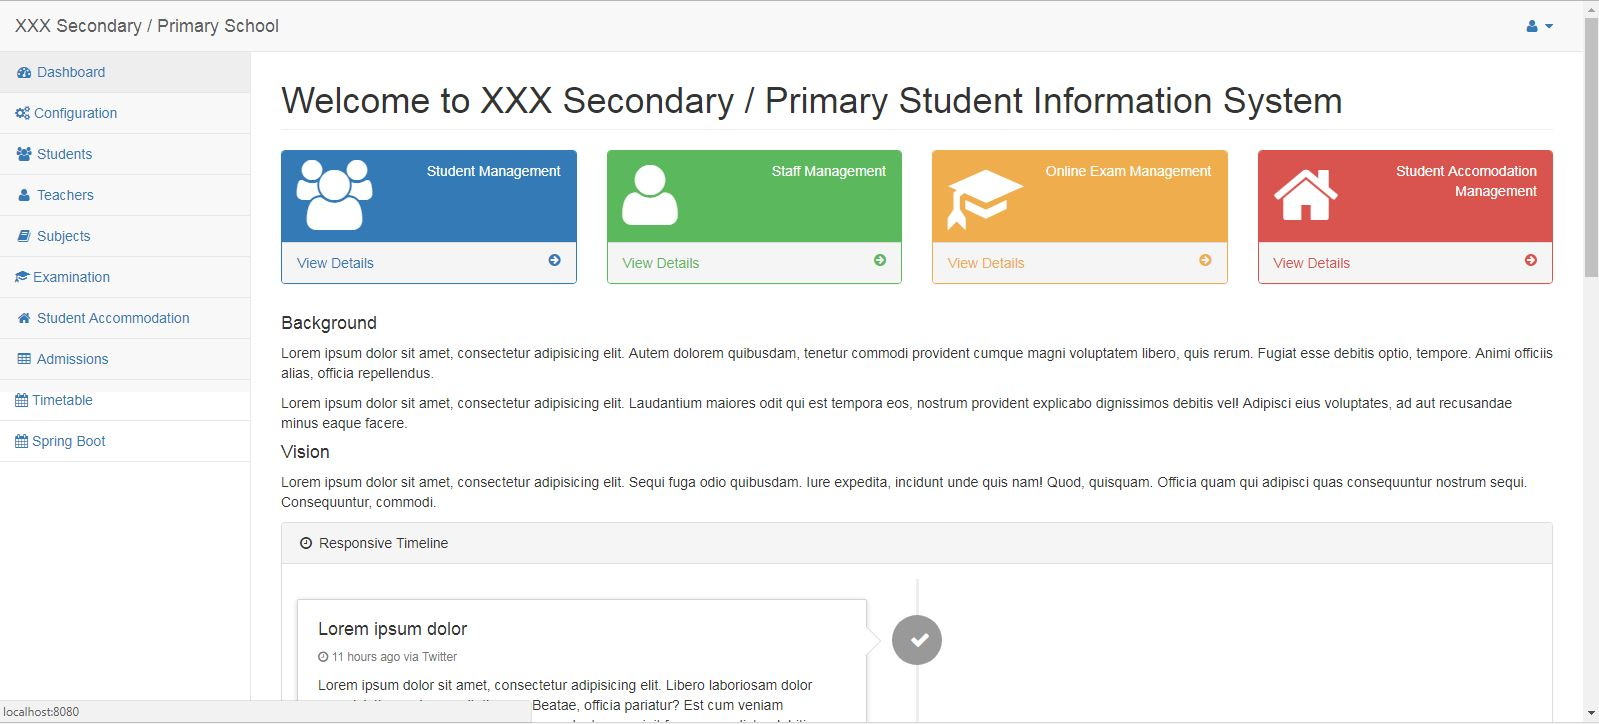
\includegraphics[height= 0.5\textheight, width = 0.5\textwidth, keepaspectratio]{sis.jpg}
			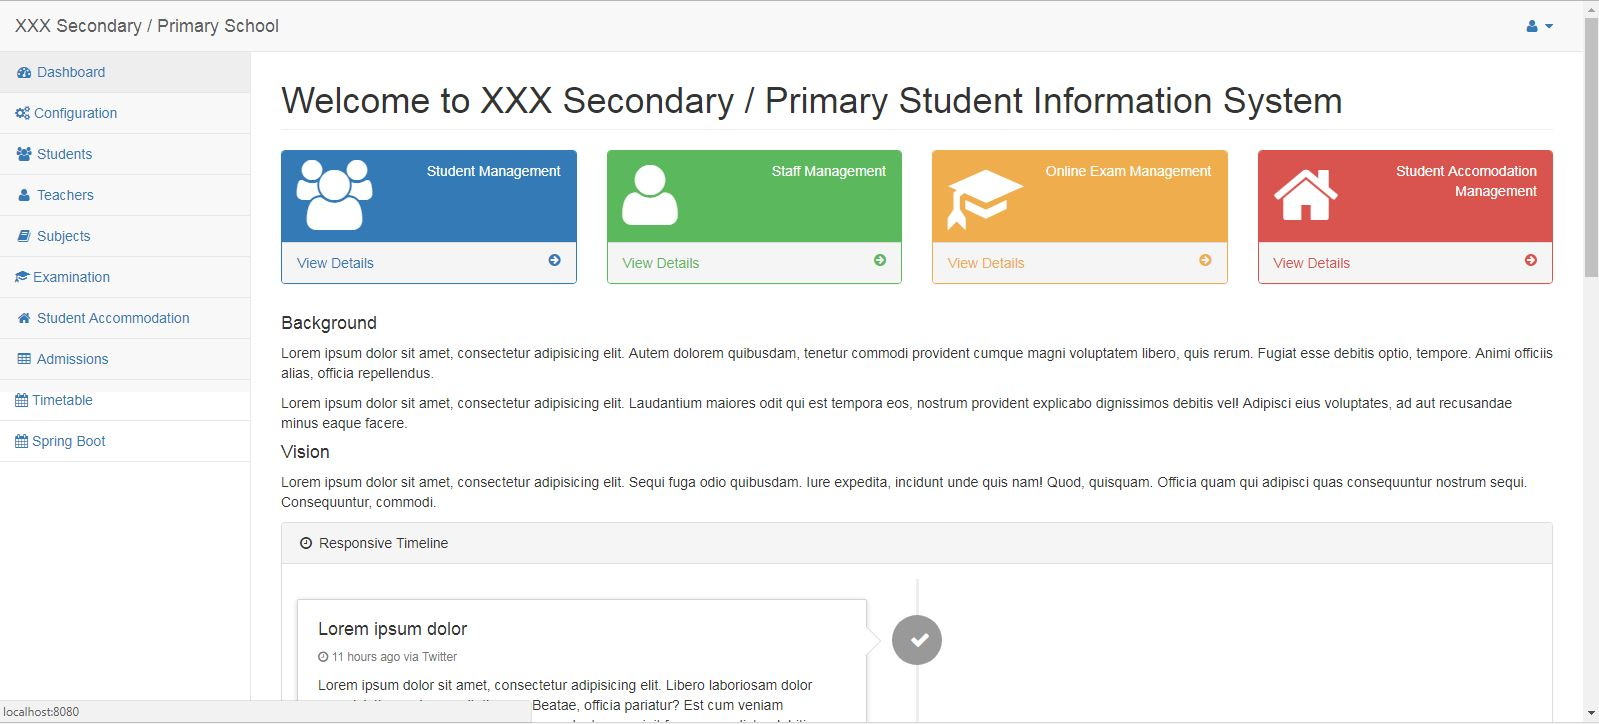
\includegraphics[height=5cm]{sis.jpg}
			\caption{This is the Home Page for SIS}
			\label{sis_home}
			
		\end{center}
	\end{figure}

	\subsection{Locating an Image in A Lower Directory}
	This Section illustrates how to reference other images that are not in the root directory of the LaTex document you are working on.
	To do that see Figure ~\ref{bts_views} Below:
	This is the total number of views for the Blood Sweat and Tears Music Video on YouTube.
	
	\begin{figure}[htbp]
		\begin{center}
			
			% 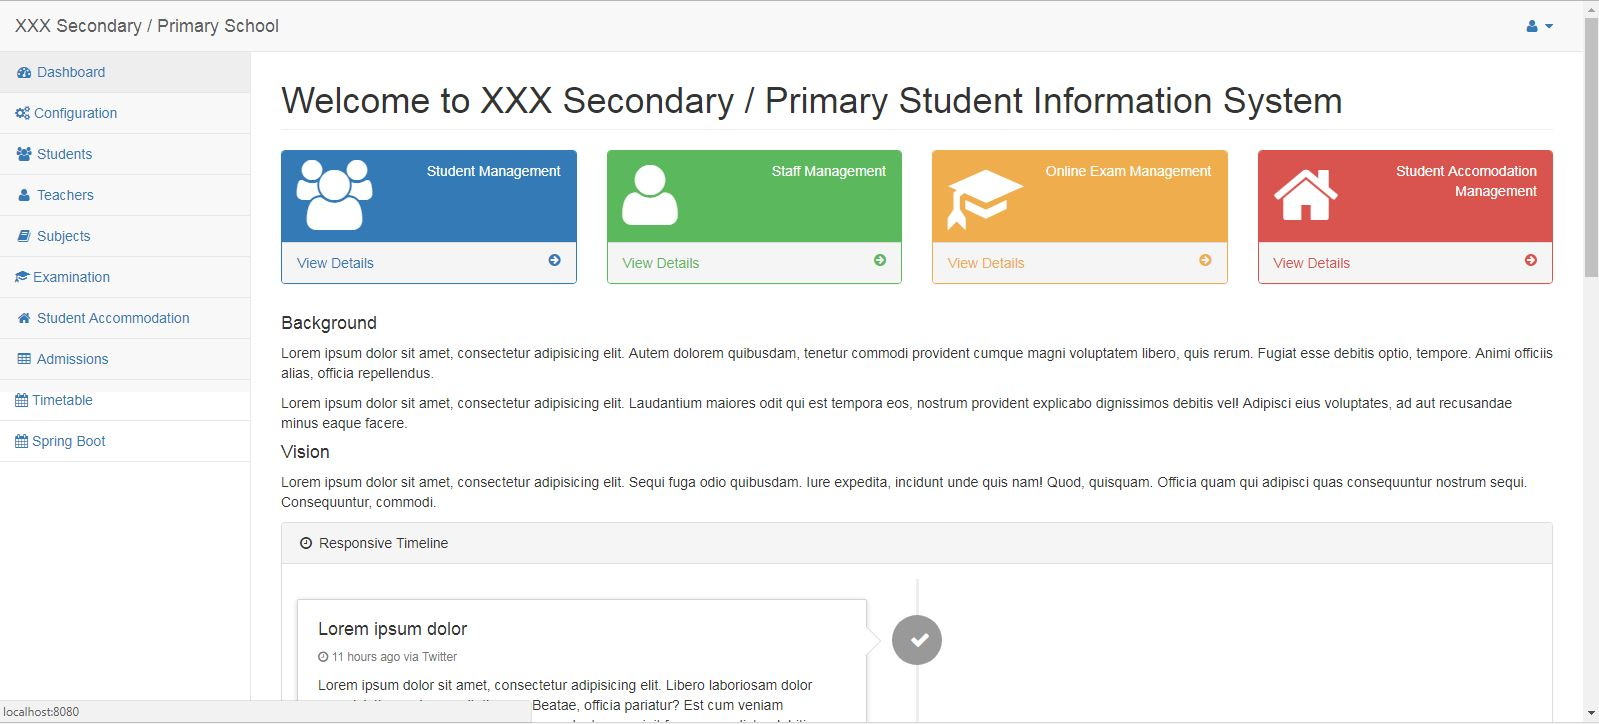
\includegraphics[height= 0.5\textheight, width = 0.5\textwidth, keepaspectratio]{sis.jpg}
			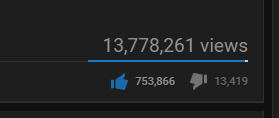
\includegraphics[height=5cm]{img/bts.png}
			\caption{ BST View Count}
			\label{bts_views}
			
		\end{center}
	\end{figure}

	\subsection{Locating Images in A Higher Directory Level}
	The two examples shown so far are used to locate images in the current working directory bas well as the lower level directory meaning a directory with a sub directory. Here the example shows how to include images from a higher level directory. See Figure ~\ref{car_image}
	
		\begin{figure}[htbp]
		\begin{center}
			
			% 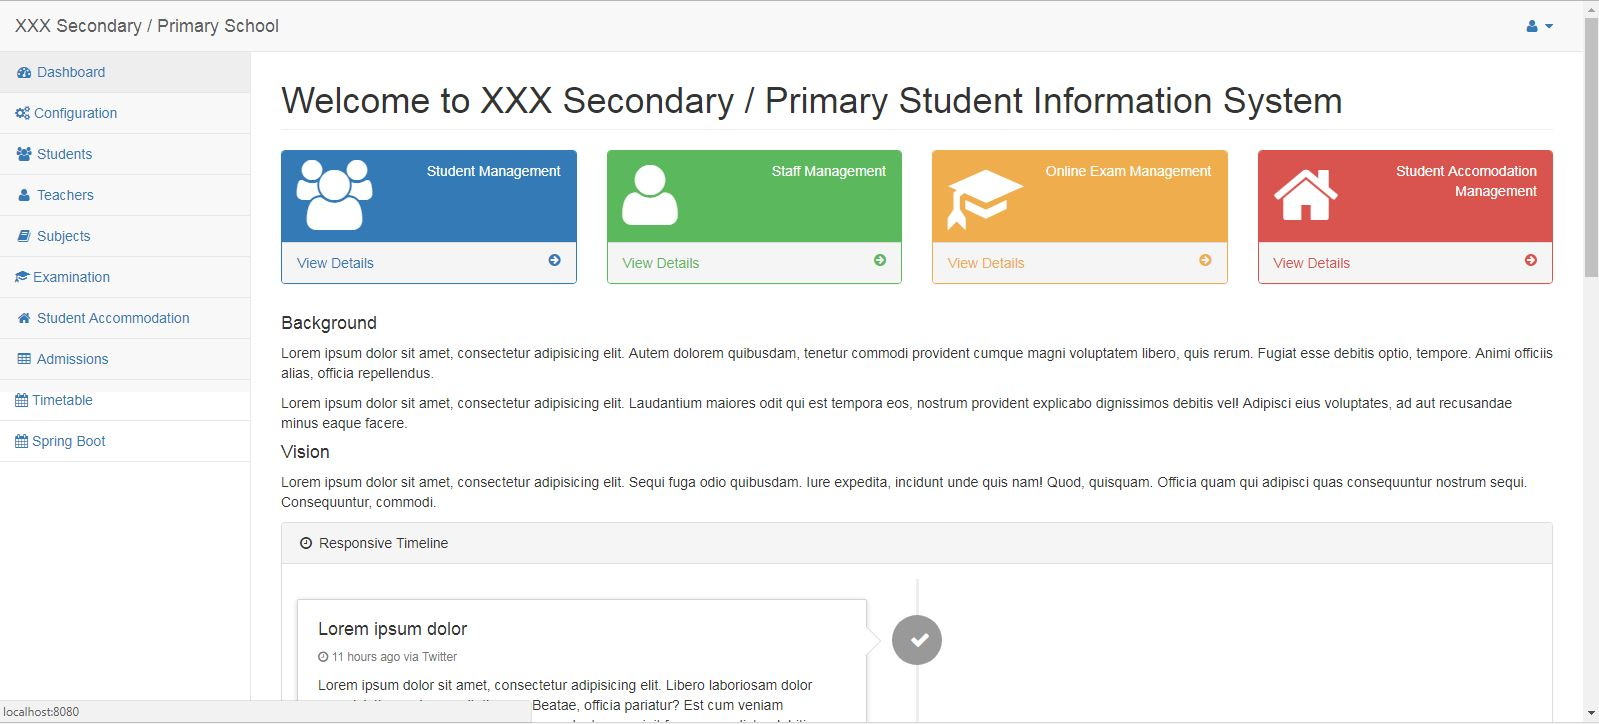
\includegraphics[height= 0.5\textheight, width = 0.5\textwidth, keepaspectratio]{sis.jpg}
			\includegraphics[height=5cm]{../Images/car.png}
			\caption{ Facebook Car Game using Gifs}
			\label{car_image}
			
		\end{center}
	\end{figure}
	
	

	

	
\end{document}	